\chapter{Assignment B: Satellite Coordinates from Kepler Elements}
The main objective of the assignment is to know how to compute and predict the satellites' position by using Kepler elements.

\section{Theory}
According to~\cite{misra2006global}, the orbital position of one satellite can be computed with
\begin{align}
	n &= \sqrt{\frac{GM}{a^3}} \\
	M & = n(t-t_p) \\
	M & = E-esinE \\
	\mathbf{r}&=\left[\begin{matrix}
		acosE-ae \\
		a\sqrt{1-e^2}sinE \\
		0 \\
	\end{matrix}\right]
\end{align}
where, $n$ is the mean motion, $GM$ is the earth's gravitational constant $3986004.418*10^8\ m/s^2$, $a$ is the length of the semi-major axis of ellipsoid ($6378137.0$ m), $e$ is the eccentricity of the ellipsoid calculated by $e^2=2f-f^2$ with $f$ being the flattening ($\frac{1}{298.257223563}$). \\
The transformation from the orbital coordinate frame to the ECEF coordinate frame can be computed using the inclination $i$, the right ascension of the ascending node $\Omega$ and the argument of perigee $\omega$.
\begin{equation}
\mathbf{r}_{ECEF}=\mathbf{R}(-\Omega)\mathbf{R}(-i)\mathbf{R}(-\omega)\mathbf{r}_{orbit}
\end{equation}

\section{Tasks}
\begin{itemize}
	\item Implement a \textsc{Matlab} function for estimating satellite positions in the orbital coordinate system.
	\item Convert the positions to the inertial system.
	\item Visualization of satellite positions for an interval.
\end{itemize}
\section{Code}
Complementary functions: \\
\textbf{deg2rad: conversion from degree to radian} as previous one. \\
\textbf{rad2deg: conversion from radian to degree} as previous one. \\
\textbf{consR: construct a rotation matrix}:
\lstinputlisting{../../assignment/utils/consR.m}
\textbf{estimateEccAnomaly: estimate eccentric anomaly}:
\lstinputlisting{../../assignment/utils/estimateEccAnomaly.m}
\textbf{lutOmegaAndAnomaly: lookup ascension and anomaly}:
\lstinputlisting{../../assignment/utils/lutOmegaAndAnomaly.m}
\textbf{calcSatPosition: compute satellite positions}:
\lstinputlisting{../../assignment/utils/calcSatPosition.m}
\textbf{ExampleHelperSat: visualization.}:
\lstinputlisting{../../assignment/ex2/ExampleHelperSat.m}
\textbf{Entry}:
\lstinputlisting{../../assignment/ex2/ex2_satellite_position_calc.m}
\begin{figure}[h]
	\centering
	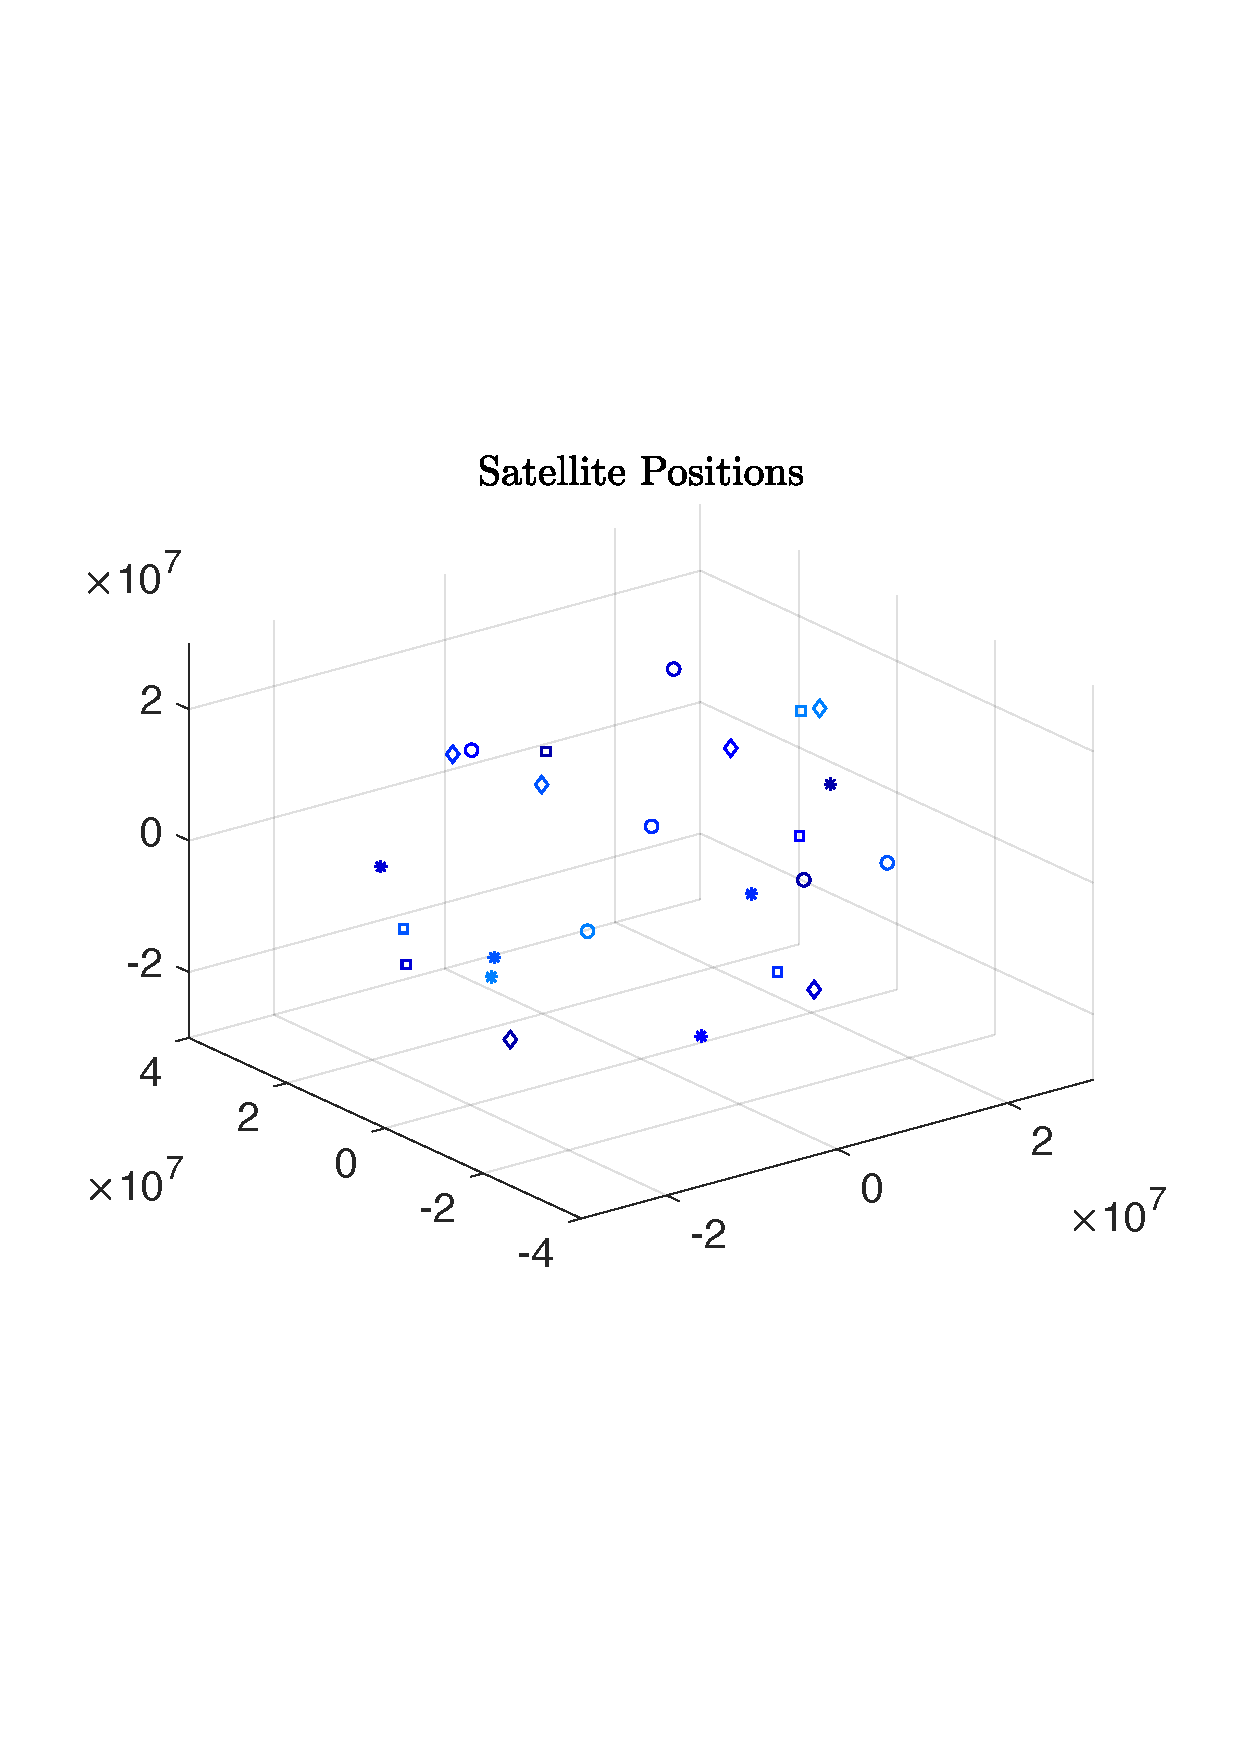
\includegraphics[width=\textwidth]{figures/ex21}
	\caption{Satellite Positions at given epoch.}
	\label{fig:ex2_1}
\end{figure}

\begin{figure}[h]
	\centering
	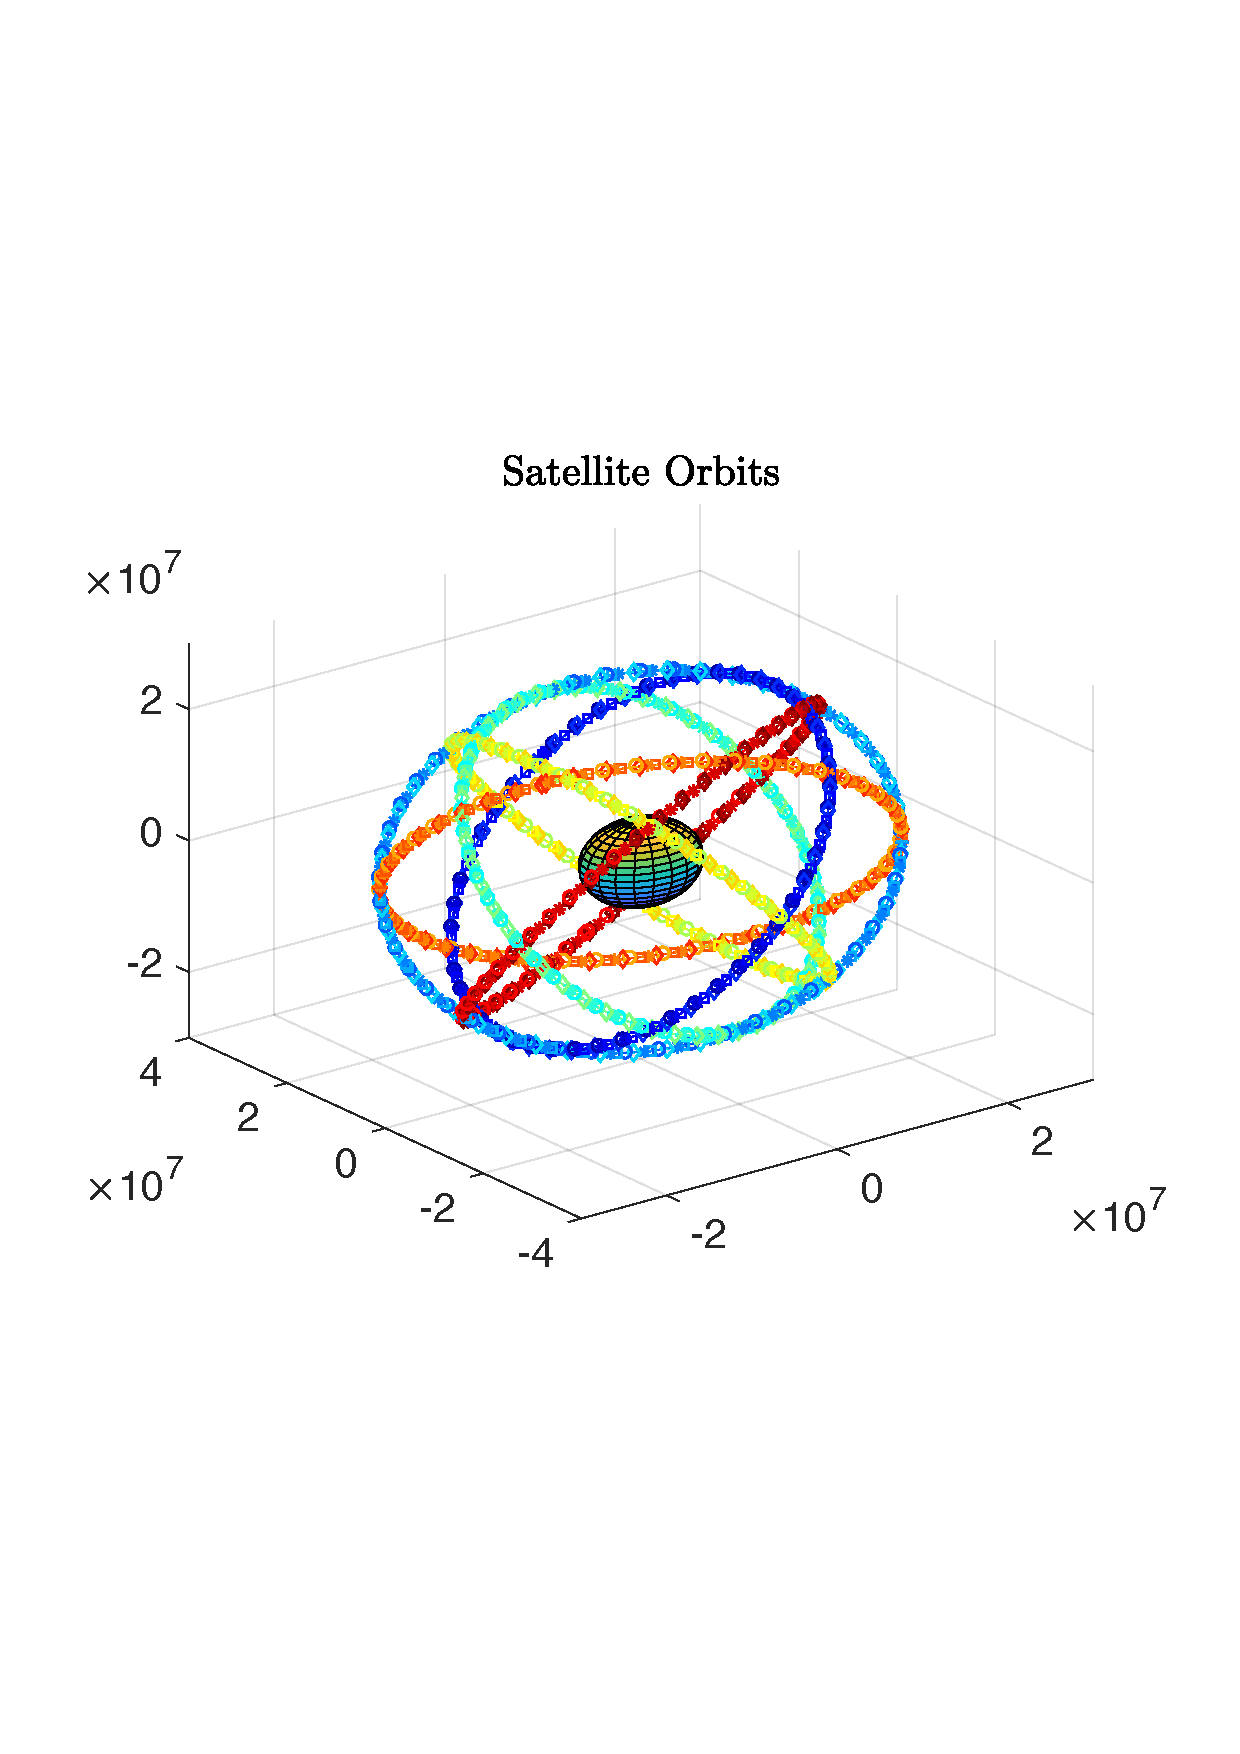
\includegraphics[width=.8\textwidth]{figures/ex22}
	\caption{Satellite orbits for 12 hours.}
	\label{fig:ex2_2}
\end{figure}
\section{Experiments}
\subsection{Single Epoch}
The result is shown in Fig~\ref{fig:ex2_1}
\subsection{Time Interval}
The result is shown in Fig~\ref{fig:ex2_2}
\subsection{DEMO Video}
A animation that demonstrates the motion of 24 satellites can be watched by the following link: \url{https://youtu.be/PjKFGVKaSvQ}.
\subsection{Conclusion}
Through this assignment, I grasp how to do the predictions of satellite positions using the Kepler elements.
